\documentclass{report}

\usepackage[utf8]{inputenc}
\usepackage[frenchb]{babel}
\usepackage[T1]{fontenc}
\usepackage{lmodern}

\usepackage{a4wide}

\usepackage{pstricks}
\usepackage{graphicx}

\usepackage[colorlinks, linkcolor=blue]{hyperref}


\begin{document}

\section{Rendu 2D}

	\subsection{Introduction - Le Tile Mapping}
	
		Le Tile mapping est une methode de rendu utilisée dans de nombreux jeux où les textures affichées
		se repetaient constamment, comme le montre l'image ci-dessous.
		
		$\,$
		
		\begin{center}
			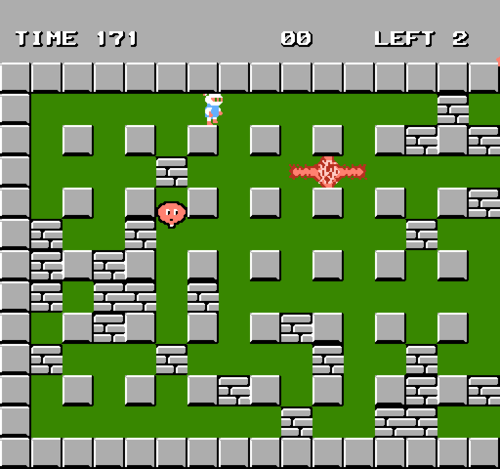
\includegraphics[width=10cm]{./img/bomberman.png}		
		\end{center}
		
		Le concept de Tile Mapping est de coller côte à côte des "tiles" (tuiles en anglais) dans une zone régulière.
		Pour cela, nous subdivisons l'écran en une grille régulière et mettons une image dans chacune des cases de cette grille.
	
	\subsection{Coût mémoire}
		
		L'avantage ici et qu'au lieu de définir une texture représentant la carte complète nous définissons une grille de $n*m$ cases.
	
	\subsection{Principes}
	
		
		Le principe du Tile Mapping est d'associer à chaque image affichée un entier la repésentant.
		

	\subsection{Detection de collisions}

\end{document}